\documentclass[digital, oneside, table, nolot, nolof]{fithesis4}
%\documentclass[printed, twoside, table, nolot, nolof]{fithesis4}

%% The following section sets up the locales used in the thesis.
\usepackage[resetfonts]{cmap}
\usepackage[T1]{fontenc}
\usepackage[main=english, czech]{babel}

%% The following section sets up the metadata of the thesis.
\thesissetup{
    date          = \the\year/\the\month/\the\day,
    university    = mu,
    faculty       = fi,
    type          = bc,
    department    = Department of Machine Learning and Data Processing,
    author        = Veronika Burgerová,
    gender        = f,
    advisor       = {RNDr. Zuzana Nevěřilová, Ph.D.},
    title         = {Conversion between First-person and Third-person Narratives},
    TeXtitle      = {Conversion between First-person and Third-person Narratives},
    keywords      = {nlp},
    TeXkeywords   = {nlp},
    abstract      = {Tato práce se zabývá převodem literárního textu mezi ich-formou a er-formou. Cílem je vytvořit nástroj, který převádí texty mezi oběma oběma formami. V práci se zaměřuji na shrnutí základů teorie vyprávění a syntaktických struktur odlišujících ich-formu a er-formu. Na základě těchto informací navrhuji sadu pravidel pro zajištění převodu, popisuji implementaci nástroje provádějícího automatickou konverzi a vyhodnocuji kvalitů dosažených výsledků.

In this thesis, I explore the topic of the conversion between first-person and third-person narratives. The aim is to create a tool that converts texts between the two forms. I summarize the basics of narrative theory and the syntactic structures that distinguish the first and third person. Based on this overview, I propose a set of rules to perform the conversion, describe the implementation of a tool providing automatic conversion, and evaluate the quality of the results achieved.

},
    thanks        = {First of all, I would like to thank my advisor Zuzana Nevěřilová for helping me discover a suitable topic when I thought it was completely hopeless, for her willingness to help me, and for many valuable comments on the whole thesis.

Many thanks to Jan Michael Kormaník, Jan Horáček, and Laura Ondušková for proofreading and feedback on the text of the thesis. I also thank all the external evaluators and authors who provided their texts.

Warm thanks to my family for their lifelong support, my friends for their encouragement, the penguins and Paštika for the daily laugh, and Schola Artist for the opportunity to hang upside down and fly away from it all on aerial silks.

Finally, I cannot put into words my gratitude to Honza Horacek for his undying support, love, care, and unimaginable tolerance. I am grateful to have converted this person into my person.
},
    bib           = bibliography.bib,
    %titleEn       = {Design and implementation of a new MTBbus protocol},
    %TeXtitleEn    = {Design and implementation of a new MTBbus protocol},
    %keywordsEn    = {bus, mtb, rs485, embedded, stm32, C++, qt, protocol, avr, arm, kicad},
    %TeXkeywordsEn = {bus, mtb, rs485, embedded, stm32, C++, qt, protocol, avr, arm, kicad},
    %assignment    = {data/zadani_ofic.pdf},
    facultyLogo = fithesis-fi,
}
\usepackage{makeidx}      %% The `makeidx` package contains
\makeindex                %% helper commands for index typesetting.
\usepackage[acronym]{glossaries}          %% The `glossaries` package
\renewcommand*\glspostdescription{\hfill} %% contains helper commands
\loadglsentries{example-terms-abbrs.tex}  %% for typesetting glossaries
%\makenoidxglossaries                      %% and lists of abbreviations.
\makeglossaries
%% These additional packages are used within the document:
\usepackage{paralist} %% Compact list environments
\usepackage{amsmath}  %% Mathematics
\usepackage{amsthm}
\usepackage{amsfonts}
\usepackage{url}      %% Hyperlinks
\usepackage{listings} %% Source code highlighting
\lstset{
  basicstyle      = \ttfamily,
  identifierstyle = \color{black},
  keywordstyle    = \color{blue},
  keywordstyle    = {[2]\color{cyan}},
  stringstyle     = \color{teal},
  commentstyle    = \itshape\color{magenta},
  breaklines      = true,
}
\usepackage{floatrow} %% Putting captions above tables
\floatsetup[table]{capposition=top}
\usepackage[babel]{csquotes} %% Context-sensitive quotation marks

\usepackage[font=itshape]{quoting}
\begin{document}

% Highlight overfulls
\setlength{\overfullrule}{5pt} % TODO: remove

\chapter{Introduction} \label{chap:uvod}
According to scientific estimates, the written word appeared around 3000 BC. The beginnings of the written word gave people the ability to put stories, which until then had only been spread orally, on paper (or its historical equivalent). And this is where the history of creative writing begins. During the millennia, the process of writing evolved. Thanks to the written language, a drafting process was enabled for storytellers.

With the invention of computers, much of the writing process has been automated. Today, we have: the ability to efficiently rewrite a text, functions as Find \& Replace, editors that perform automatic grammar correction, webpages that allow people to collaborate online, word counters, and many other tools that affect the creative process of how the books are being written.

In my eighteen years of writing experience, I have spoken to hundreds of people from the writing community, watching the issues, ideas, and thought processes they -- we -- are dealing with during the drafting process. And there is a question often asked: \emph{how} to write the story? In what person? Who should be the narrator? Sometimes, the writers even rewrite the text to the other person to be able to compare both versions. That made me ask myself another question: could computers also handle this problem?

This thesis aims to automate the process of person change and implement a tool that would convert a written text between first-person and third-person narratives. This conversion covers the grammatical aspects of these narratives. To achieve this goal, I have designed and implemented a rule-based system. That includes an implementation of a tool \emph{RephrasErIch}, proposing several conversion rules for both directions, and then implementing these rules into the tool.

In the second chapter, I briefly summarize the existing solutions for my problem. In the third chapter, I introduce some important terms of the narrative theory and describe the impacts of conversion on a given text's narrative features. \textbf{TODO four, syntactic strucutres}. Chapter five contains an overview of the proposed rules accompanied by diagrams for illustration. In chapter six, I introduce the tool itself. I speak about external tools that I have used for the \emph{RephrasErIch} implementation and then describe the system's design and some important classes.

To assess the tool's performance, I have evaluated it on text data. The evaluation process and its results are described in chapter seven. Afterward, I discuss the errors and the possibility (or impossibility) of solving those errors.

I conclude my thesis with a summarization of achieved results, suggestions for future work, and usage of the implemented tool.



\chapter{State of the art} \label{chap:state-of-art}
So far, the task of the narrative mode conversion is largely unexplored. There are many open problems in the area of \emph{natural language processing} (NLP), and text rephrasing, in general, is one of them. Besides, there is a specific challenge to face in NLP: several solutions to any NLP task are language-specific. Naturally, most of the research which can be found on any topic is performed on English. Processing of the English language has several advantages: it has far fewer word forms and there is much more of the available textual data in English. These factors make the data more representative, In contrast, Czech morphology is more complex, and due to the number of speakers, there are not many researchers dealing with the NLP  of the Czech language. Since I have chosen to work with Czech texts in this thesis, I have to face this specific challenge as well.

This leads me to the fact that there is no existing solution to this task for Czech. However, there are tools that solve at least some parts of the problem, or similar problems, such as text paraphrasing.

Generalizing the problem to any language, only few papers on this topic are found, as expected, all for English.

In this chapter, at first, I introduce the existing solutions for the English language, and then I examine the situation in the Czech processing. TODO

\section{Existing Solutions for English}

As mentioned in the previous chapter, my motivation for this task is to create a tool for writers. However, previous work on this topic has mostly focused on a different goal: to convert the person in replies provided by virtual assistants (VA), such as Siri, Alexa, or Google Assistant. Due to the difference in the target application, these solutions address some problems that are irrelevant to our case and neglect several subtasks related to the creative writing process.

The system designed by Lee et al. \cite{lee2020converting} focused on spoken messages in VA-assisted conversations. To the best of our knowledge, this is the first attempt at Point of View (POV) conversion. The authors have developed several models that can be classified by two main approaches: rule-based and machine learning. The rule-based model works with a set of rules which describe how the grammatical conversion should be performed. The model relies on a classification model that provides Named Entity Recognition (NER), which is already implemented in the VA. In addition, the model uses a Part Of Speech (POS) tagger and a constituency parser.

Besides the rule-based model, several deep learning based models have been developed. These models were trained on data collection provided by Amazon Mechanical Turk workers. According to the evaluation results, the deep learning based models have better performance.

Recently, another effort has been published by Granero Moya and Oikonomu Filandras \cite{granero-moya-oikonomou-filandras-2021-taking}. Their research also focuses on virtual assistant technologies. Unlike our work and the work of Lee et al. they focus on conversion in only one direction: third-person to first-person. They also worked with the two approaches and developed a rule-based model and a deep learning system. Their deep learning models show better results than the rule-based model, which served as a baseline here, as well.

\section{Tools for Czech}

In the introduction to this chapter, I explained that there is currently no solution to this problem for Czech. Nevertheless, I will briefly introduce a few tools that address more general problems.

\subsection{Morphological analyzers}

Morphological analysis is an essential part of NLP. In the context of narrative mode conversion, it cannot be done without morphological analysis. For instance, the person of a word being processed needs to be known, and a morphological analyzer can provide the tags describing the grammatical categories of the word.

There are several tools in the Czech community providing morphological analysis.

\paragraph{Ajka}

is one of the first morphological analyzers for Czech. Currently, Ajka is no longer in development and has been replaced by the new morphological analyzer Majka. \cite{Sedlacekthesis}

\paragraph{Majka}

is a fast morphological analyzer developed at Masaryk University. The implementation builds on the previous system, Ajka, but it is faster and more flexible. Majka is based on finite automata, and it works with a morphological database. At the moment, the author provides databases not only for Czech but also for other languages. The tool is able to assign lemmas and tags to the analyzed word form, generate all word forms of a given lemma and generate a word form based on the given lemma and tags. \cite{majka}

\paragraph{Morfo} is a system developed at Charles University, which provides morphological analysis using a large morphological dictionary. \cite{morfo}


\subsection{Morphological taggers}

Morphological disambiguation, also called tagging, reduces the output of morphological analysis to a single base shape and a single tag that are valid for a token in a particular context.

\paragraph{MorphoDiTa} (Morphological Dictionary and Tagger) is a tool developed at Charles University that performs morphological analysis, morphological generation and tagging. \cite{strakova14}

\paragraph{Desamb} is a morphological tagger developed at Masaryk University, which combines rule-based and statistical methods. \cite{desamb2010}


\subsection{Syntactic analyzers}
\label{sec:synt-an}

In addition to morphology, there is another linguistic level that we need to deal with in order to perform POV conversion: syntax. In order to rephrase a sentence, syntactic analysis is required. The syntactic analysis is preceeded by morphological analysis. Let's take a look at some existing syntactic analyzers for Czech.

\paragraph{SYNT} is a syntactic analyzer developed at the NLP Centre at Masaryk University. The tool is based on Czech meta-grammar, and it was designed for morphologically-rich languages.

\paragraph{SET} (Syntactic Engineering Tool), also developed at the NLP Centre, is implementing a new approach to the syntactic analysis of Czech. This new approach is based on pattern recognition. \cite{set}

\paragraph{UDPipe} is a pipeline from Charles University, which performs tagging, lemmatization and syntactic analysis utilizing neural networks. \cite{straka-2018-udpipe}

\subsection*{Note on the tools listed}

When analysing a text, we usually proceed in order from the lowest levels of language exploration to the higher ones. Therefore, the tools mentioned above are often plugged into pipelines one after the other.



\chapter{Narrative theory} \label{chap:teorie-vypraveni}
\emph{Narratology}, or narrative theory, is a literary science that has experienced considerable development over the last hundred years. The topic of narrative theory has been explored by literary theorists across Europe throughout the twentieth century. Consequently, a number of different typologies and proposals have emerged on how to view the topic of narrative and narrative mode, and how to conduct narrative analysis.

.\cite{kubicek-vypravec}

In this chapter I introduce some basic narratological concepts. Next, I show a selected typology to demonstrate its relevance to this thesis, ????? and focus on the application of narrative theory to creative writing.

\section{Foundations of Literary Theory and Narratology}

\subsection{Point of view}

Pojem \emph{point of view} lze do češtiny přeložit jako \emph{hledisko}. Hledisko je

TODO najít tu knihu s definicemi pojmů!

\subsection{Forms of narrative by person}

\emph{Person} is a linguistic category of verbs, on the basis of which the primary forms of narrative are distinguished.In addition to verbs, this form is also manifested in personal and possessive pronouns and some special conjunctions.
\paragraph{Ich-forma}

TODO kniha s definicemi

\paragraph{Du-forma}

\paragraph{Er-forma}

\subsection{System of narrative modes}

From a number of narrative typologies I decided to choose the system proposed by Czech linguist and literary theorist Lubomír Doležel. Doležel's system of narrative modes is captured in the tree diagram in the figure \ref{fig:schema-dolezel}.\cite{dolezel-narativni-zpusoby}

\begin{figure}[ht]
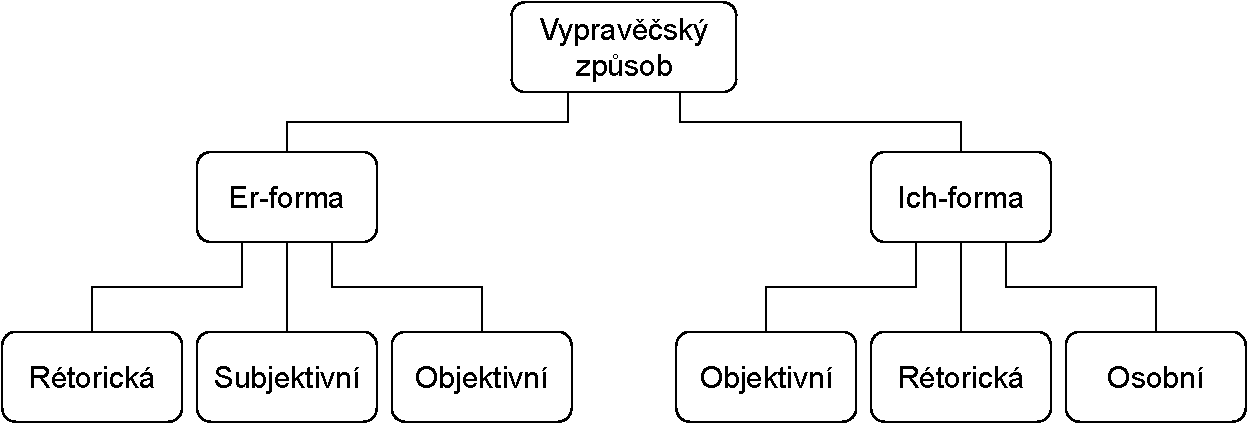
\includegraphics[width=1\textwidth]{data/dolezel-schema.pdf}
\caption{System of narrative modes by Doležel}
\label{fig:schema-dolezel}
\end{figure}





\chapter{Conclusion} \label{chap:zaver}
The aim of this thesis was to explore the topic of person transfer and implement a tool that will transfer texts between the first-person and third-person narratives.
To achieve these goals, I have compiled an overview of the topic from the perspective of literary theory and Czech grammar. Based on this information, I proposed several rules for conversion in both directions. Subsequently, I implemented these rules in the RephrasErIch tool I created. Finally, I evaluated the tool's results on a set of textual data.



\printbibliography

\appendix
\chapter{Appendix} \label{chap:appendix}
The attachment \texttt{rerich.zip} contains:

\begin{itemize}
	\item Directory \texttt{rerich} which consists of:
	\begin{itemize}
		\item Directory \texttt{classes} containing implemented classes mentioned in Chapter \ref{chap:rerich}.
		\item Directory \texttt{enums} with enumeration classes.
		\item Directory \texttt{tools} containg classes providing the communication with external tools.
		\item Files \texttt{erich-rules.py} and \texttt{icher-rules.py} with implementation of the rules described in Chapter \ref{chap:navrh-pravidel}.
		\item File \texttt{utils.py} with some utility functions.
		\item File \texttt{main.py} for running the tool.
	\end{itemize}
	\item File \texttt{aara-rerich.py} which contains a slightly modified implementation of \texttt{Aara}.
\end{itemize}


\end{document}
